\section{Plasticine Specialization for RNN Serving} \label{sec:rnn_arch}

Recurrent Neural Networks (RNNs) are a class of sequence models that plays a key role
  in low-latency,
  AI-powered services in datacenters \cite{fowers2018configurable, jouppi2017datacenter}.
In these services,
  the platforms assume that user requests come in individual samples
  and need to be served with very stringent latency window
  for real-time human computer interaction.
  An example of such workload is
  Google Translate, where inference happens concurrently when a user types.
Despite its popularity, RNN model serving is hard to accelerate efficiently.
Modern software and hardware platforms support optimized BLAS routines.

An efficient execution of RNN requires flexibility in supporting more than BLAS kernels, 

Low-precision inference are commonly used to reduce memory footprint of deep learning models and
increase compute density of hardware accelerators.
Plasticine, however, only supports 32-bit operations and datapath.
Using RNN serving as a motivating example, this section discusses the necessary architecture augmentation and
specialization needed to efficiently map real-time inference on Plasticine.

In \Cref{sec:lowprec}, we propose the necessary micro-architectural changes to
  support low-precision arithmetics on Plasticine.
We also discuss architectural parameter selection for Plasticine
  to serve RNN applications efficiently in \Cref{sec:sizing}

\subsection{Mixed-Precision Support} \label{sec:lowprec}
\label{sec:arch:varprec}
Previous works \cite{fowers2018configurable, jouppi2017datacenter}
  have shown that low-precision inference can deliver promising performance
  improvements without sacrificing accuracy.
In the context of reconfigurable architectures such as FPGAs,
  low-precision inference not only increases compute density,
  but also reduces required on-chip capacity for
  storing weights and intermediate data.

To support low-precision arithmetics without sacrificing coarse-grained reconfigurability,
we introduce two low-precision struct types in Spatial: a tuple of 4 8-bit and 2 16-bit floating-point 
numbers, \texttt{4-float8} and \texttt{2-float16} respectively.
Both types packs multiple low-precision values into a single precision storage.
We support only 8 and 16-bit precisions, which are commonly seen in deep learning inference hardwares.
Users can only access values that are 32-bit aligned.
This constraint guarantees that the microarchitectual change is only local to the PCU.
Banking and DRAM access granularity remains intact from the original design.

\begin{figure}
  \centering
  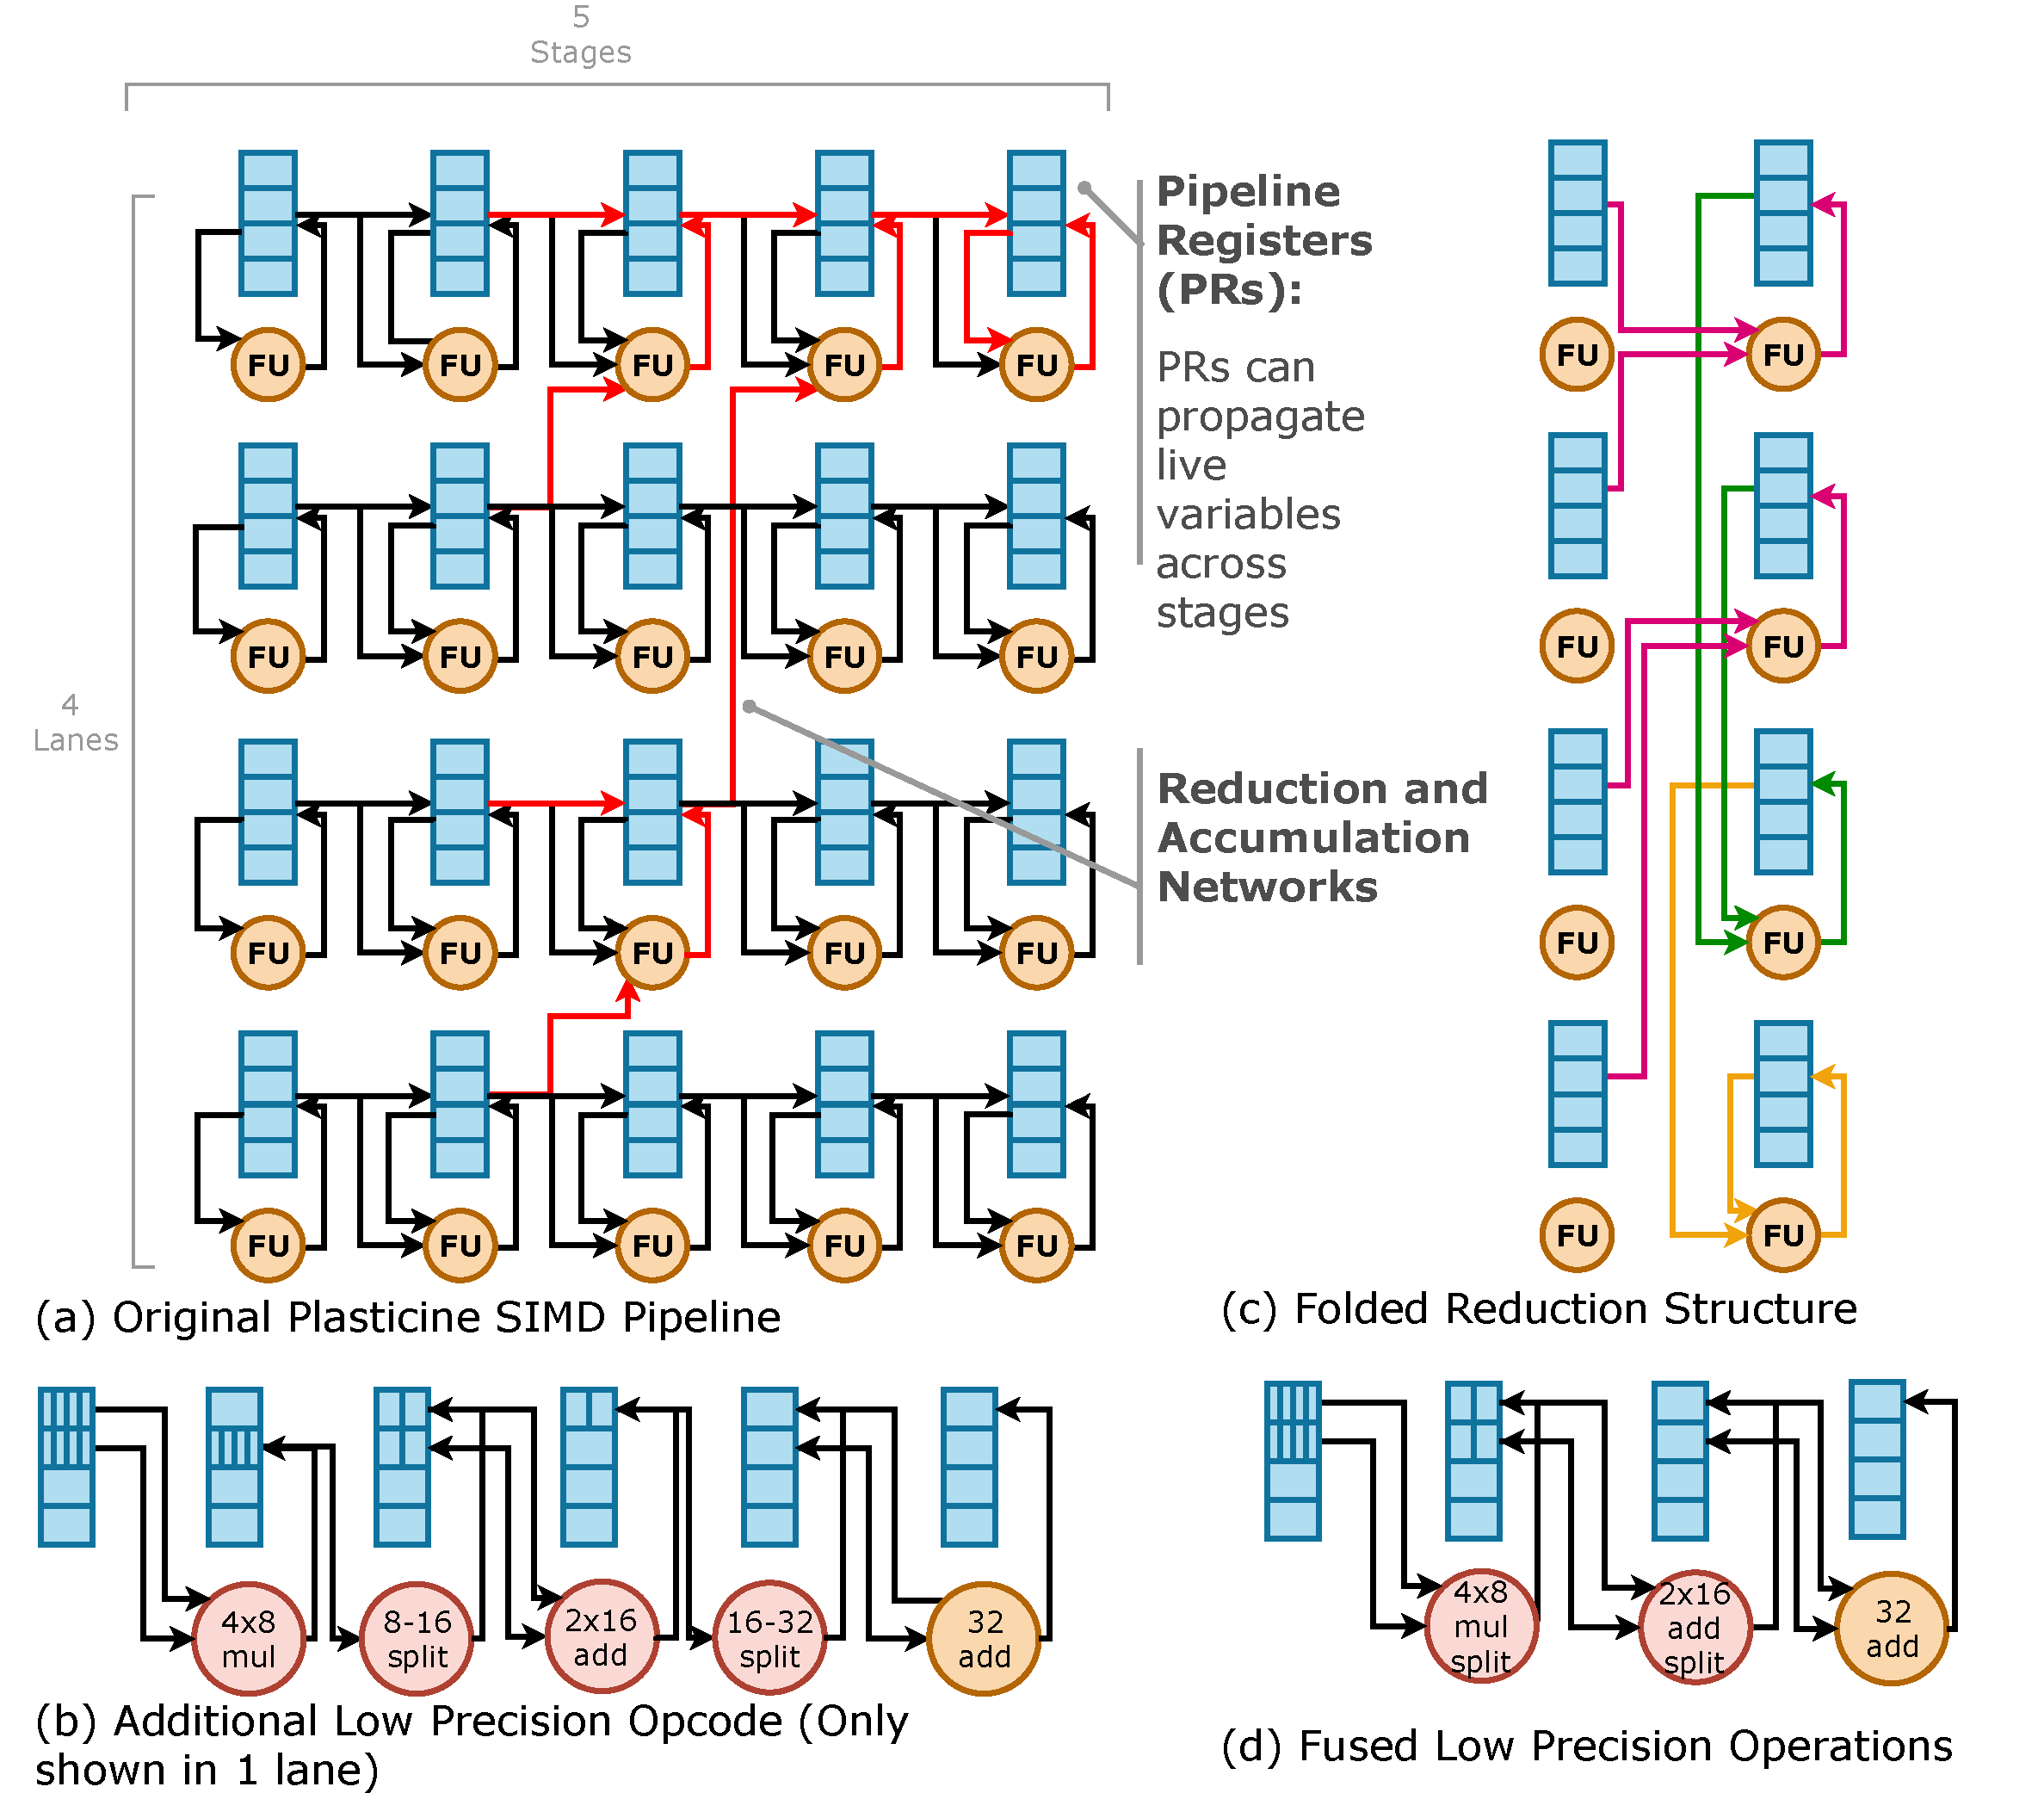
\includegraphics[width=1\columnwidth]{figs/lowprec.pdf}
  \caption{Plasticine PCU SIMD pipeline and low-precision support.
  Red circles are the new operations. Yellow circles are the original opertaions in Plasticine.
  In (d) the first stage is fused $1^{st}, 2^{nd}$ stages, and the second stage is fused
  $3^{nd}$, $4^{th}$ stages of (b).
   }
  \label{fig:lowprec}
  \vspace*{-0.3in}
\end{figure}
Figure \ref{fig:lowprec} (a) shows the original SIMD pipeline in a Plasticine PCU.
Each FU supports both floating-point and fix-point operations.
When mapping applications on Plasticine,
  the inner most loop body is vectorized across the lanes of the
SIMD pipeline, and different operations of the loop body are mapped to different stages.
Each pipeline stage contains a few pipeline registers (PRs)
  that allow propagation of live variables across stages.
%The PRs are accessible as both inputs and outputs of the FU.
%An FU can also read previous stage's PRs
%as its input value.
Special cross-lane connections as shown in red in Figure \ref{fig:lowprec} enable reduction operations.
To support 8-bit element-wise multiplication and 16-bit reduction, we add 4 opcodes to the FU, shown in
Figure \ref{fig:lowprec} (b).
The $1^{st}$ and $3^{rd}$ stages are element-wise, low-precision operations
  that multiply and add 4 8-bit and 2 16-bit values, respectively.
The $2^{nd}$ and $4^{th}$ stages rearrange low-precision values into two registers,
  and then pad them to higher precisions.
The $5^{th}$ stage reduces the two 32-bit value to a single 32-bit value using the existing add operation. 
From here, we can use the original
reduction network shown in Figure \ref{fig:lowprec} (a) to complete the remaining reduction and accumulates
in 32-bit connection.

With 4 lanes and 5 stages,
  a PCU first reads 16 8-bit values,
  performs 8-bit multiplication followed by rearrangement and padding,
  and then produce 16 16-bit values after the second stage.
The intermediate values are stored in 2 PRs per lane.
Next, 16 16-bit values are reduced to 8 16-bit values
  and then rearranged to 8 32-bit value in 2 PRs per lane.
Then, the element-wise addition in 32-bit value
  reduces the two registers in each line into 4 32-bit values.
These values are fed through the
  reduction network that completes the remaining
  reduction and accumulation in two plus one stages.

In a more aggressive specialization,
  we can fuse the multiply and rearange into the same stage.
We also fuse the first low-precision reduction with the next rearange as shown in Figure \ref{fig:lowprec} (d).
In this way, we can perform the entire low-precision map-reduce in 2 stages
  in addition to the original full precision reduction.
In order to maximize hardware reuse,
  we assume that it is possible to construct a full precision FU
  using low-precision FUs.
In addition, we observe that the original reduction network in the SIMD lanes
  could lead to low FU utilization.
To improve FU utilization, we fold the entire tree structure in a single stage.
Figure \ref{fig:lowprec} (c) shows the folded reduction accumulation structure.
Specifically, latter reductions in the tree are mapped to earlier stages in the pipeline.
In this setup, the entire reduction plus accumulation
  is still fully pipelined in $\log_2(\#_{LANE})+1$ cycles
  with no structural hazard.
With fused reduced-precision multiplication and reduction, and folded reduction tree,
  a PCU is able to perform all map-reduce that accumulates $4 \#_{LANE}$
  8-bit values using 4 stages.
All the operations are completed in $2+\log_2(\#_{LANE})+1$ cycles.

\subsection{Sizing Plasticine for RNN Serving} \label{sec:sizing}
Evaluating an RNN cell containing $N$ hidden units and $N$ input features
  requires $2N^2$ computations and $N^2+N$ memory reads.
With large $N$, the compute to memory ratio is 2:1.
The original Plasticine architecture uses a checkerboard layout
  with 1 to 1 ratio between PCU and PMU.
A PCU has 6 stages and 16 lanes, and a PMU has 16 banks.
This provides a 6:1 ratio between
  compute resource and on-chip memory read bandwidth.
As a result of this layout,
  on-chip memory read bandwidth becomes the bottleneck for accelerating RNN serving applications.
Given that RNNs cover a wide range of important applications,
  we select a Plasticine configuration tailored for RNN serving.
Specifically, we choose a 2 to 1 PMU-PCU ratio with 4 stages in each PCU.
Figure \ref{fig:arch} shows the layout of this Plasticine variant.
\begin{figure}
  \centering
  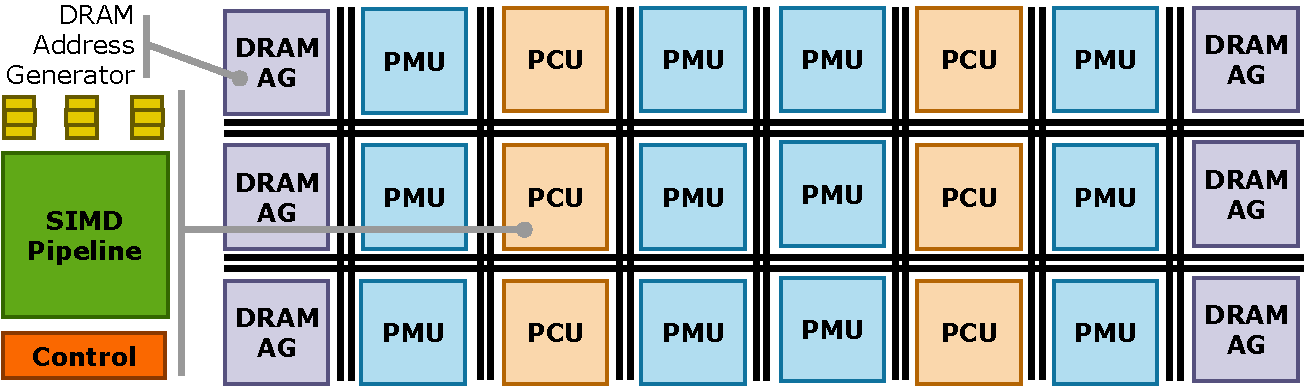
\includegraphics[width=\columnwidth]{figs/arch.pdf}
  \caption{Variant configuration of Plasticine for serving RNN.}
  \label{fig:arch}
  \vspace*{-0.2in}
\end{figure}
